% \documentclass[10pt, oneside, english]{article}   	
\documentclass[10pt, oneside]{article}
\usepackage{geometry}                		
\geometry{a4paper}                   		
% \usepackage[english, es-noindentfirst]{babel}
% \selectlanguage{english}
\usepackage[utf8]{inputenc}               		
\usepackage{graphicx}			
\usepackage{amssymb}
\usepackage{authblk}
\usepackage{multicol}
\usepackage{rotating}
\usepackage{capt-of}
\usepackage{hyperref}	%autoref
\usepackage{amsmath}	%equation*
\newenvironment{Figure}
	{\par\medskip\noindent\minipage{\linewidth}}
	{\endminipage\par\medskip}

\title{Word embeddings for predicting political affiliation based on Twitter data}

\author[]{Ibrahim Abdelaziz}
\author[]{Oliver Berg}
\author[]{Angjela Davitkova}
\author[]{Venkatesh Iyer}
\author[]{Shriram Selvakumar}
\author[]{Kumar Shridhar}
\author[]{Saurabh Varshneya}
\affil[1]{Technische Universität Kaiserslautern}

\date{\today}


\begin{document}
\maketitle
\begin{multicols}{2}


\section{Abstract}

Twitter as one of today's biggest social media platforms allows political figures to express their thinking easily and with a concise message. We propose a generic way of classifying political affiliation based on Twitter posts. This involves Word2Vec vector representations of the input data and utilizes pre-trained embeddings for the German language. With this we have shown to be capable of insightfully position German political figures in the political spectrum. 


\section{Introduction}

Social media platforms like \emph{Twitter} allows people of interest to communicate their personal opinion, and as such e.g. indicating political alignment, through a comprised message being only a few hundred character long. This yields broad potential to characterize personality traits such as political affiliation on.

Generally speaking, political motives were shown to be consistently predictable with an accuracy better than chance already \cite{Biessmann2017}.
This paper therefore proposes a \emph{deep learning} based classification model together with \emph{word embeddings} \cite{Pelevinala2016}. This allows a later analysis to find interesting constellations within the (German) political spectrum.
We leverage word embeddings to represent words in context. We thereby restrict ourselves to pre-trained models. Subsequently, a convolutional neural network (CNN) holistically classifies the Twitter profile by assigning each Twitter message a separate party label and combining these into a complete class score.


\section{Related Work}

Today, sentiment classification is mostly done using recurrent- or convolutional neural networks as described in \cite{Kim2014}. The presented approach uses a basic CNN trained on pre-trained word vector representations and does only little hyperparameter tuning to already achieve compelling results in question classification.

Additionally, \cite{Misra2016} introduces Recurrent Neural Networks (RNNs) for political bias analysis. Intuitively, RNNs operate more similar to how humans tend to process language: word by word, forming sentences. RNNs do train slower when compared to CNNs though, and CNNs generally produce more efficient representations of the data.

In connection to the given focus of working on Twitter data, \cite{Cohen2013} further introduces interesting questions concerning applicability of classification onto real data outside the training samples. It depicts the validation process as being prone to optimistic interpretations of the result when overlooking problems in latent attribute inference. This also suggests a critical view on this paper's final analysis results. 

In addition, \cite{SuggestedAdditionalResource2018} motivates context- and time dependencies within political data, which again makes analyzing an overall corpus of Twitter data a broadly connected issue.


\section{Methodology}

Formally, this paper proposes work on classifying Twitter data of political figures and picturing tendencies and dependencies within the data. As such, the following methodology is being applied. 

\subsection{Dataset} 

The dataset used in this approach was constructed of German politicians' Tweets posted on their Twitter accounts. 1000 German politicians' profiles with attributes "person name", "political party" and "twitter username" were retrieved from the website “https://www.wahl.de/”.
To reduce noise, only politicians belonging to the seven major political parties with respect to parliament activities, namely "CDU", "CSU", SPD", "FDP", "GRÜNE", "LINKE" and "AFD", are considered.

After the filtering stage this leaves a list of around 800 politicians, 125 of them are separated for the testing dataset. For each one up to 1000 of his/her most recent Tweets are gathered using Twitter API.

To prepare the Tweets for the training, and testing steps, each Tweet was preprocessed by first removing URLs, special characters, user names, and mentions. Then output empty Tweets are removed, and all characters are masked and put to lowercase.

Given the difference in the number of Tweets for each party, and in order to create a balanced training dataset, each party is restricted to a total of 12000 Tweets for training dataset, where each politician contributes approximately the same number of Tweets.

To represent the preprocessed Tweets text into numerical values that can be used to train, and test our model a pre-trained Word2Vec model is used \cite{DBLP:journals/corr/abs-1301-3781} - pre-trained on 200 million German Tweets \cite{cieliebak2017twitter} - which represent each word of the Tweet as a 200-dimensional vector.

\subsection{Classification}

The 200-dimensional word vectors are fed to a CNN model for classification.
The employed CNN architecture, shown in \autoref{fig:cnnArchitecture},  is based on \cite{Kim2014} which uses its model for sentiment analysis specifically. We used the implementation of this paper provided on github to train our own model on Tensorflow by finetuning the hyper-parameters and adding dynamic learning rate for our classification problem.

The first layers embeds words into low-dimensional vectors. Subsequent layers performs convolutions over the embedded word vectors using multiple filter sizes; sliding over 3, 4 and 5 words at a time. Max-pooling transforms the result of the constitutional layer into a long feature vector, dropout regularization with keep probability 0.5 is added and the result is classified using a final softmax-layer. We employed a dynamic learning rate between 0.005 to 0.0001 with exponential decay coefficient of 2.5 applied every epoch.

\begin{Figure}
	\centering
	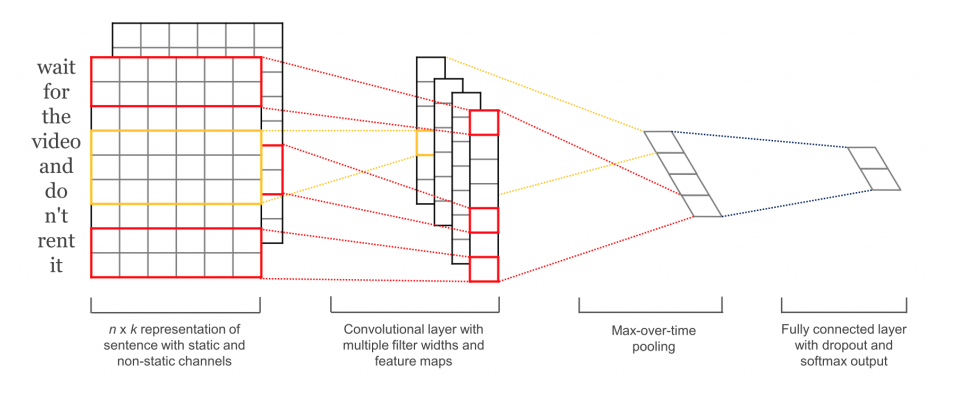
\includegraphics[width=\linewidth]{images/cnn_architecture1.png}
	\captionof{figure}{Model Architecture \cite{Wildml2015}}
	\label{fig:cnnArchitecture}
\end{Figure}

The overall classification process can be sub-divided into two elementary parts: First we \textbf{feed input data} to the neural network to then \textbf{classifying the (test-)data} for their respective classes.

In order to feed input data: For each party a raw text collection of all Tweets is considered. For each line - containing a single Tweet - a $<$PAD$>$ tokens is appended to achieve a fixed size length of size 35 which is the maximum word-length in a tweet for our dataset.  A vocabulary built on the complete corpus of existing words within the data maps each word to an integer between 0 and 109933 (number of existing words) for faster indexing.
Note that each Tweet is now represented as a vector of integers only. Using the pre-trained Word2Vec model, each Tweet can then be represented as a Matrix $M \in \mathbb{R}^{35 \times 200}$.

For classifying the user Tweets to the correct political party, we then feed the batches of twitter data along with their correct political party one-hot-encoded labels and train the above defined CNN. To optimize the network we use cross entropy loss defined as
\begin{equation*}
	H_{y'}(y) = - \sum_{i} y'_{i} \log (y_{i})
\end{equation*}
where $y$ is our predicted probability distribution, and $y'$ is the true distribution (the one-hot vector with the true-class party labels). 


\section{Qualitative Analysis}

For a quantitative analysis of the results, every Tweets are taken as sentences and a sentence vector of the same dimension as the word vectors used for training (i.e. 200 dimensional vector) is constructed. In doing so, the Tweet is tokenized into words and every word's corresponding token vectors are taken from the word embedding space. A sentence embedding vector is constructed by adding the word vectors and dividing them by the number of words. Note that only those Tweets for which all its words were present in the word embedding space are considered and that any Tweets with \emph{UNK} token were ignored for a cleaner analysis. This effectively removes any Tweets that were not completely related to political topics such as simple link- or hashtag-forwarding. 


\subsection{Visualization}

For the visualization of results, sentence vectors were visualized using a Tensorflow built-in visualizer called the Embedding Projector that allows interactive visualization and analysis of high-dimensional data.
The high-dimensional vectors is reduced to 2 dimensional space using TSNE and then the model is further visualized. However, the visualizations over word-embeddings of tweets lacked clear distinction between political party clusters. 

We found several reasons for this:
Since a user Re-Tweets other parties Tweets with his opinions, it could be that subjects get mixed rather quickly across parties.
Another reason for such mixed clusters could be the fact that any collection of party-members is typically tweeting about similar issues with some in favor of and some against some specific proposition, which may lead to strictly disconnected sentiment groups within the same party.

As such, a direct embedding as described earlier did not prove to be a good measure to visualize the result. This motivates our usage of the ``political compass'' \cite{PoliticalCompass2017} for visualizing the result further. 

For the political compass representation, we use a four way graph plot with attributes of ``Left-wing'' and ``Right-wing'' on the X-axis (Economic Scale), as well as ``Authoritarian'' and ``Libertarian'' on the Y-axis (Social Scale). Each party is positioned on the compass by a given X,Y coordinates.

To visualize the results and to compare whether the user has been classified to it’s correct class, we need to plot each user's position on the compass. This was achieved through following steps:
\begin{enumerate}
	\item Passing all of a user's Tweets to the classification model as specified above in the model architecture section
	\item Obtaining the party classification for each Tweet by getting the party with highest probability
	\item For each party count the number of Tweets classified to this party
	\item Averaging all Tweets counters to get one vector representing the distribution over all classes
	\item Compute x,y coordinates as a weighted sum of the vector distribution multiplied by X,Y vectors coordinates of the seven parties
\end{enumerate}

\subsection{Inference}

The subsequent visualization was created as described in above section.

\begin{Figure}
	\centering
	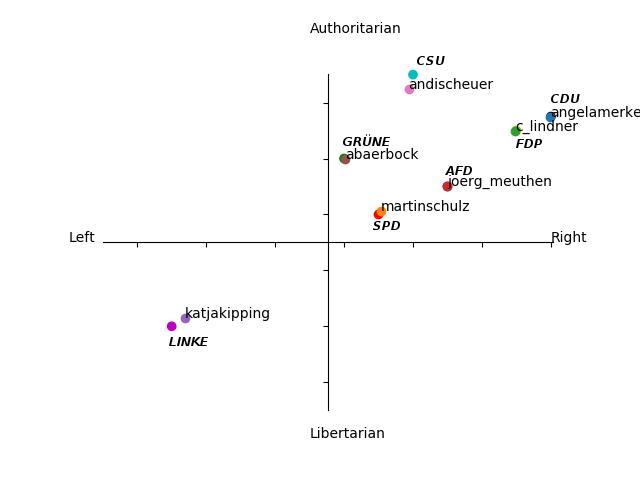
\includegraphics[width=\linewidth]{images/Political_Compass-final.png}
	\captionof{figure}{Plotting on Political Compass}
	\label{fig:political_compass}
\end{Figure}



From this depiction within the political compass, we can derive the following:

\begin{enumerate}
	\item Users generally appear close to their respective political party. As an example, we have depicted the leader of each party on political compass in \autoref{fig:political_compass}. Position of all users is provided in the implementation \footnote{ The plots of all the users are available at \url{https://github.com/rngShard/ML1_Team02/tree/saurabh-classification/src/text-classification-on-embedding/plots}  } and here a subset is plotted to avoid clutter.
	\item The FDP-class is plotted close to the CDU-class. Both party's ideology are traditionally quite similar, which matches the visualization.
	\item Few users were misclassified near other party clusters. Upon analyzing the data, we observed a common occurrence  of Tweets in the English language, which led to a huge number of $<$UNK$>$ token generation, hence the classification may not be correct. Also, total number of tweets for those users were low. After manually cleaning the data, and thresholding the minimum number of tweets to 100, we were able to see the user's plot moving to the correct classes.
	\iffalse
	\item The user ``AxelVossMdEP'' from the party CDU was found to appear very close to Die Grünen. In our context, this indicates a strong affiliation towards Die Grünen instead of CDU. Upon analyzing the data, we observed a common occurrence  of Tweets in the English language, which will have led to a huge number of $<$UNK$>$ token generation, hence the classification may not be correct. After manually cleaning the data, we were able to see the user's plot moving to the correct class CDU.
	\fi
\end{enumerate}

\section{Results}
Classification to a specific party based on a single tweet is a difficult task, even for humans. We, through our experiments comprehend the same as our results on individual tweets gave a low classification accuracy of 55 percent.
However, taking majority voting over a set of tweets for a specific user led to a considerable increase in the classification accuracy depicted below:
\begin{center}
	\begin{tabular}{|l|l|l|l|}
	\hline
	\textbf{party} & \textbf{users} & \textbf{max tweets/user} & \textbf{accuracy} \\ \hline
	AFD & 25 & 200 & 92 \\
	CSU & 25 & 200 & 84 \\
	FDP & 25 & 200 & 80 \\
	Grüne & 25 & 200 & 72 \\
	Linke & 25 & 200 & 88 \\
	SPD & 25 & 200 & 84 \\
	CDU & 25 & 200 & 72 \\
	\hline
	\end{tabular}
\end{center}


\section{Conclusion}

As we have shown, a comparably simple convolutional neural network is able to nicely separate political figures concerning party affiliation. Interesting findings like single entities more closely connecting to general party-affiliated language or specifically different language have been pointed out.

As the underlying word embeddings are taken from the German-language Wikipedia dump, we are currently restricted to German-language Tweets as well as to overall German-language features. This does suffice for general classification purposes, but poses the additional question of how the analysis would be affected if the embeddings were to be taken from \emph{intrinsically political} data samples. 
Also, our approach primarily focuses on CNNs and proves them to be efficient already. For future work, it would be intriguing to compare the capabilities of RNNs or other topologically different architectures. 


\end{multicols}

\bibliography{lit}
\bibliographystyle{apalike}

\end{document} 
